%! TeX program = lualatex
\documentclass[main]{subfiles}

\begin{document}

\providecommand{\confB}[1]{{\conf}^{[#1]}}  % batch slot: lambda^[k]

\title[AutoML: BO]{Bayesian Optimization}
\subtitle{Parallel Bayesian Optimization}
\author[Bernd Bischl]{Bernd Bischl}
\date{}

\titlebackground*{images/AutoML_HPO_bayesian3.jpg}

    \maketitle


\begin{frame}[t]{Why Parallel BO?}
  \begin{itemize}
    \item Modern compute is inherently \textbf{parallel} 
    \item Cores, nodes, GPUs sit idle if BO runs strictly one eval at a time
    \item We can try to fully parallelize the underlying objective $\cost(\conf)$,
      and in ML there are good chances this is possible
    \item Still attractive to generate a \textbf{batch} of $q > 1$ points to evaluate \textbf{simultaneously}
    \item Trade-off: more wall-clock speedup vs.\ fewer feedback rounds / less optimally placed points
    \item But remember: random search sometimes hard to beat
  \end{itemize}
\end{frame}


\begin{frame}[t]{The Core Challenge}
  \small
  \begin{itemize}
    \item Acquisition function $\acq(\conf)$ is designed for \textbf{one} candidate at a time
    \item Naively proposing the top-$q$ maximizers of $\acq$ gives \textbf{near-duplicates}: they cluster around the current global peak of $\acq$ $\leadsto$ wastes $q-1$ of the $q$ evaluations
    \item We need batch proposals that are simultaneously \textbf{informative} and \textbf{diverse}
  \end{itemize}
  \begin{center}
    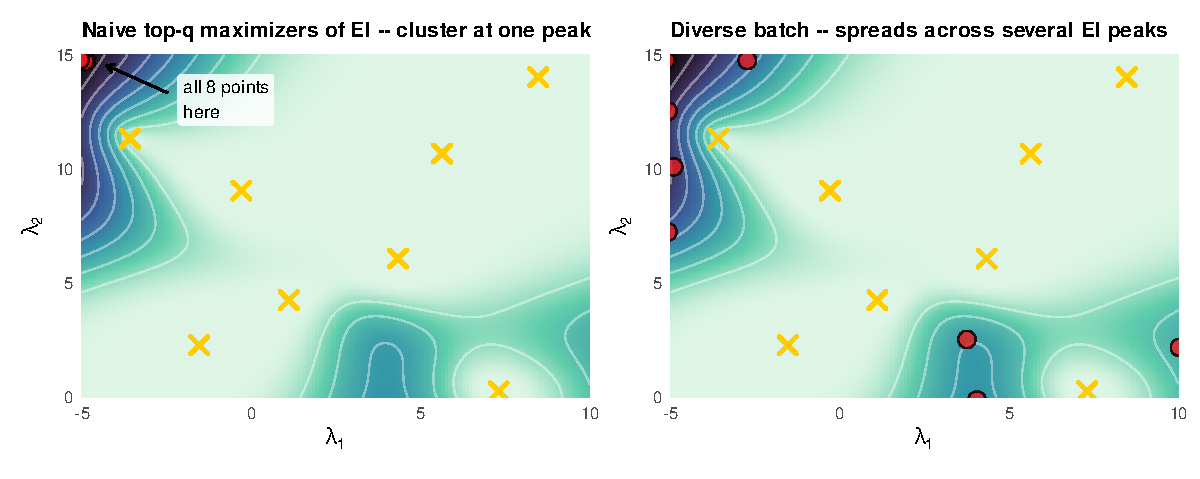
\includegraphics[width=0.55\textwidth]{images/08_batch_bo_naive_vs_diverse.pdf}\\
    \footnotesize EI on Branin after 8 initial evals (yellow); proposed batch ($q=8$, red). \\
    Naive top-$q$ collapses onto one peak; a diverse batch spreads across several.
  \end{center}
\end{frame}


\begin{frame}[t]{Joint / $q$-Acquisition Functions}
  \begin{itemize}
    \item Extend acquisition to \emph{joint} criterion over batch $\batchconf = (\confB{1}, \ldots, \confB{q})$:
        % $$\acq_q(\batchconf) = \E_{Y(\confB{1}), \ldots, Y(\confB{q})}\big[\, g(Y(\confB{1}), \ldots, Y(\confB{q}))\,\big]$$
    \item Example: $q$-expected improvement~\liturl{Wang et al. 2020}{https://arxiv.org/abs/1602.05149}
        $$\qEI(\batchconf) = \E\!\left[\max_{k=1,\ldots,q} \max\!\left(\cmin - Y(\confB{k}),\,0\right)\right]$$
    \item Reward the \textbf{best} outcome in the batch -- naturally encourages diversity
    \item No closed form; estimated via \textbf{Monte Carlo} samples from joint posterior
    \item \textbf{Optimization:} inner problem is now $q \cdot \pcsdim$-dimensional.
    Reparameterization trick used in BoTorch 
    so $\qEI(\batchconf)$ becomes a deterministic, smooth function of $\batchconf$
    $\leadsto$ optimize with Adam / L-BFGS-B. Feasible up to $q \le 32$.
  \end{itemize}
\end{frame}


\begin{frame}[t]{Kriging Believer / Fantasizing}
  \footnotesize
  Iteratively fill the batch~\liturl{Ginsbourger et al. 2010}{https://link.springer.com/chapter/10.1007/978-3-642-10701-6_6}:
  \begin{itemize}
    \item Start with current surrogate; propose $\confB{1} \in \argmax \acq(\conf)$
    \item \textbf{Fantasize} the outcome at $\confB{1}$: replace the unknown $\cost(\confB{1})$ with
        \begin{itemize}
            \item Kriging believer: posterior \textbf{mean} $\surro(\confB{1})$
            \item Constant liar: fixed value, e.g., $\min_t \cost(\confI{t})$ or $\max_t \cost(\confI{t})$ from archive
            \item MC fantasizing: sample from the posterior
        \end{itemize}
    \item Refit and propose $\confB{2} \in \argmax \acq(\conf)$; repeat until $q$ points assembled
  \end{itemize}
  \textbf{Effect:} fantasy eval lowers post. unc. around $\confB{k}$ $\leadsto$ EI collapses there $\leadsto$ next peak elsewhere
  \begin{center}
    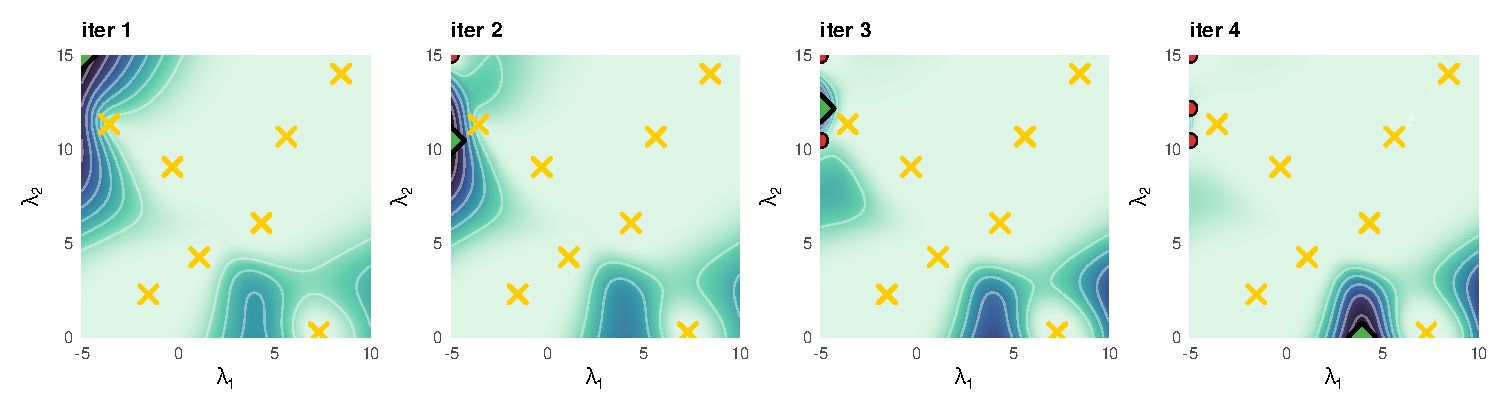
\includegraphics[width=0.55\textwidth]{images/08_batch_bo_kriging_believer.pdf}\\
    \footnotesize Kriging believer on Branin-EI ($q=4$): yellow $\times$ = initial design, red = earlier picks, green $\diamond$ = current pick
  \end{center}
\end{frame}


% \begin{frame}[t]{Heuristic 2: Local Penalization}
%   \begin{itemize}
%     \item After selecting $\confB{k}$, multiply the acquisition function by a \textbf{penalty} ~\liturl{González et al. 2016}{https://proceedings.mlr.press/v51/gonzalez16a.html} that decays with distance from $\confB{k}$:
%     $$\tilde{\acq}_{k+1}(\conf) = \acq(\conf) \cdot \prod_{j=1}^k \varphi\!\left(\|\conf - \confB{j}\|\right)$$
%     \item $\varphi$ typically a logistic / soft-step function around a Lipschitz-motivated radius
%     \item Picks the next point from areas the previous ones do not already cover
%     \item Cheap to compute, no refitting needed, easy to parallelize across $q$~\liturl{González et al. 2016}{https://proceedings.mlr.press/v51/gonzalez16a.html}
%   \end{itemize}
% \end{frame}


\begin{frame}[t]{Thompson Sampling: Parallelism for Free}
  % \footnotesize
  % \begin{columns}[onlytextwidth,T]
  %   \column{.55\textwidth}
    \begin{itemize}
      \item \textbf{Thompson sampling}~\liturl{Kandasamy et al. 2018}{https://proceedings.mlr.press/v84/kandasamy18a.html}: draw a sample path $\tilde{\cost}$ from the posterior of the surrogate, propose $\argmin_{\conf} \tilde{\cost}(\conf)$
      \item Each new posterior sample gives a different proposal $\leadsto$ draw $q$ samples to get $q$ points
      \item \textbf{Batch diversity = posterior diversity:} no extra mechanism
      \item Spread when the GP is uncertain, concentrated when the posterior is peaked
      % \item Especially clean with GP surrogates (via random Fourier features) and with RF surrogates (sample a tree / a leaf distribution)
      \item Scales well with $q$; a go-to in large-batch / high-dim BO
    \end{itemize}
  %   \column{.45\textwidth}
  %   \begin{center}
  %     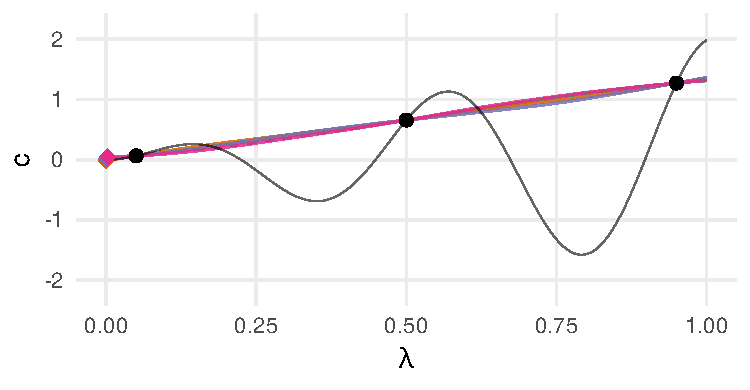
\includegraphics[width=\textwidth]{images/08_thompson_sampling.pdf}\\[0.05cm]
  %     \scriptsize $4$ posterior sample paths (colored); each path's argmin (diamond) is a Thompson proposal. Disagreement between paths $\Rightarrow$ batch diversity
  %   \end{center}
  % \end{columns}
\end{frame}


\begin{frame}[t]{Asynchronous Decentralized BO}
  \footnotesize
  \begin{itemize}
    \item Synchronous batches stall the slowest worker\\
     $\Rightarrow$ idle compute under heterogeneous runtimes.
    \item Asynchronous decentralized BO~\liturl{Egele et al. 2023}{https://arxiv.org/abs/2207.00479} avoids this
    \item Keep all $q$ workers busy at all times; react \textbf{per completion}, not per batch
    \item All workers share the same archive, fit surrogate, propose and eval
    \item On finished eval: update surrogate with the \textbf{one} new observation and propose \textbf{one} new point
  \end{itemize}
% ADBO topology: workers connected to a shared archive. Each worker sends its
% completed observation up; the archive (refit with the new data plus fantasies
% for in-flight configs) sends a new proposal down. Used in 04_BO/08_parallel_bo.tex.
\begin{center}
\begin{tikzpicture}[font=\scriptsize,
  archive/.style={rectangle, rounded corners=4pt,
                  draw=blue!60!black, fill=blue!10, thick,
                  minimum width=4.6cm, minimum height=1.05cm, align=center},
  worker/.style ={rectangle, rounded corners=2pt,
                  draw=black!60, fill=gray!8, thick,
                  minimum width=1.7cm, minimum height=0.8cm, align=center},
  finish/.style ={->, mygreen!55!black, thick, >=latex},
  propose/.style={->, blue!60!black, thick, >=latex}]

  \node[archive] (arch) at (0, 0) {\textbf{Shared archive}\\[-1pt]\scriptsize $(\confI{t}, \costI{t})$ + fantasies of pending};

  \node[worker] (w1) at (-3.0, -2.0) {worker 1\\[-1pt]\scriptsize busy: $\confI{1}$};
  \node[worker] (w2) at ( 0.0, -2.0) {worker 2\\[-1pt]\scriptsize busy: $\confI{2}$};
  \node[worker] (w3) at ( 3.0, -2.0) {worker 3\\[-1pt]\scriptsize busy: $\confI{3}$};

  % Each pair of arrows: put (up, green) writes (lambda, cost); read (down, blue)
  % pulls the archive so the worker can refit and propose locally.
  \draw[finish ] (w1.north) to[bend left=15]
        node[midway, left=2pt, font=\tiny, color=mygreen!55!black] {put $(\conf,\cost)$} (arch.south west);
  \draw[propose] (arch.south west) to[bend left=15]
        node[midway, right=2pt, font=\tiny, color=blue!60!black] {read $\hist$} (w1.north);

  \draw[finish ] (w2.north) to[bend left=10]
        node[midway, left=2pt, font=\tiny, color=mygreen!55!black] {put $(\conf,\cost)$} (arch.south);
  \draw[propose] (arch.south) to[bend left=10]
        node[midway, right=2pt, font=\tiny, color=blue!60!black] {read $\hist$} (w2.north);

  \draw[finish ] (w3.north) to[bend right=15]
        node[midway, right=2pt, font=\tiny, color=mygreen!55!black] {put $(\conf,\cost)$} (arch.south east);
  \draw[propose] (arch.south east) to[bend right=15]
        node[midway, left=2pt, font=\tiny, color=blue!60!black] {read $\hist$} (w3.north);

  % small legend
  \node[anchor=west, align=left, font=\tiny] at (4.2, -1.0)
    {\textcolor{mygreen!55!black}{$\rightarrow$ on finish: put $(\conf,\cost)$}\\
     \textcolor{blue!60!black}{$\rightarrow$ read $\hist$, refit, propose}};
\end{tikzpicture}
\end{center}
\end{frame}


\begin{frame}[t]{Asynchronous Decentralized BO}
  \begin{itemize}
    \item Picking one point at a time risks duplicating in-flight configs
    \item Avoid duplicating a \textbf{pending} config by fantasizing its outcome in the archive, e.g.,
    by some (randomized) version of Kriging believer
    \item Fantasies inflate posterior certainty around pending points $\leadsto$ $\argmax \acq$ on other workers move elsewhere,
    so proposals stay diverse w.r.t.\ running work
    \item When the real eval returns, its fantasy is replaced by the true value and the surrogate is refit
  \end{itemize}
% ADBO Gantt-style schematic: 3 workers, in-flight (dashed) vs. finished (solid)
% configs, "now" line, and an annotation at the most recent completion.
% Used in 04_BO/08_parallel_bo.tex on the two ADBO frames.
\begin{center}
\begin{tikzpicture}[font=\scriptsize, x=0.95cm, y=0.55cm]
  \draw[->, gray!60] (0, -1.4) -- (6.4, -1.4) node[anchor=west, color=gray!80] {time};
  \draw[gray!50, dashed] (3.6, 2.0) -- (3.6, -1.3) node[anchor=north, color=gray!80] {now};
  \node[anchor=east] at (-0.1,  1.5) {worker 1};
  \node[anchor=east] at (-0.1,  0.5) {worker 2};
  \node[anchor=east] at (-0.1, -0.5) {worker 3};
  \draw[fill=blue!15, draw=blue!60!black] (0, 1.2) rectangle (1.6,  1.8) node[pos=.5] {$\confI{1}$};
  \draw[fill=blue!15, draw=blue!60!black, densely dashed] (1.7, 1.2) rectangle (3.4, 1.8)
      node[pos=.5] {$\confI{4}$};
  \draw[fill=blue!15, draw=blue!60!black] (0, 0.2) rectangle (0.9, 0.8) node[pos=.5] {$\confI{2}$};
  \draw[fill=blue!15, draw=blue!60!black, densely dashed] (1.0, 0.2) rectangle (3.4, 0.8)
      node[pos=.5] {$\confI{5}$};
  \draw[fill=blue!15, draw=blue!60!black, densely dashed] (0, -0.8) rectangle (3.4, -0.2)
      node[pos=.5] {$\confI{3}$};
  \node[anchor=west, align=left, color=mygreen!55!black] at (3.6, 0.5)
    {dashed = pending\\$\rightarrow$ fantasized};
  \draw[->, mygreen!55!black, thick] (1.65, 1.5) -- (1.7, 1.5);
  \node[anchor=south, color=mygreen!55!black] at (1.65, 1.85) {finish $\Rightarrow$ refit, propose};
\end{tikzpicture}
\end{center}
\end{frame}


\begin{frame}[t]{Summary and Discussion}
  \begin{itemize}
    \item Parallel BO proposes a batch of $q$ points to exploit parallel compute; naive top-$q$ of $\acq$ collapses to near-duplicates $\leadsto$ need explicit diversification
    \item $q$EI, Kriging believer / fantasizing, Thompson sampling as batch versions
    \item ADBO: async workflow with fantasies for pending evals;\\
    avoids idle workers under heterogeneous runtimes
    \item \textbf{Practical:} match $q$ to compute (watch the sample-efficiency tax)
    \item \textbf{Diversity sanity check:} monitor pairwise distances within batches; near-duplicates are a warning sign
  \end{itemize}
\end{frame}


\end{document}
